\documentclass[12pt]{article}

\usepackage{times} % Times New Roman font
\usepackage{graphicx} % For images
\usepackage{enumitem} % For numbered items
\usepackage{lipsum} % For dummy text
\usepackage{hyperref} % For references
\usepackage{fancyhdr} % For custom headers
\usepackage{pythonhighlight} % For Python code
\usepackage{float} % For image positioning
\usepackage{amsmath} % For math equations
\usepackage{xcolor} % For custom colors


\pagestyle{empty}
\fancyhf{}
\rhead{}
\chead{}
\lhead{}
\renewcommand{\headrulewidth}{0pt}

\begin{document}

\thispagestyle{fancy}
\rhead{Assignment 1\\COMP6528\\Computer Vision\\24S1\\u7748799\\Yichi Zhang}
\section{Task 1: Basic Image I/O}

\subsection{Question 1}
\underline{All the runnable code will be provided in the code file. Hereinafter same.}\\
\underline{Built-in function will sometimes be used to test the same with comments.}\\
\underline{Details are written in the code comments to explain the usage.}\\
\\
\quad According to section 1.1 in the code file, we can complete the save operation according to the following code.
\begin{python}
  # Load the provided images
  # (I change their name to XXXX_original.jpg to avoid confusion)
  image1 = cv2.imread('image1_original.jpg')
  image2 = cv2.imread('image2_original.jpg')
  image3 = cv2.imread('image3_original.jpg')

  # Resize the images to 1024 x 720
  image1 = cv2.resize(image1, (1024, 720))
  image2 = cv2.resize(image2, (1024, 720))
  image3 = cv2.resize(image3, (1024, 720))

  # Save the resized images as JPG files
  cv2.imwrite('image1.jpg', image1)
  cv2.imwrite('image2.jpg', image2)
  cv2.imwrite('image3.jpg', image3)
\end{python}
% Leave blank if not responding to a particular question or task

\subsection{Question 2}

% Documentation, observations, results, analysis, etc.
\renewcommand{\thesubsubsection}{\thesubsection.\alph{subsubsection}}

\subsubsection{}
\quad According to section 1.2.a in the code file, we can complete the cut and save operation according to the following code.
\begin{python}
  # (a) Read image and resize
  image1 = cv2.imread('image1.jpg')
  image1 = cv2.resize(image1, (384, 256))
\end{python}


\subsubsection{}


\quad According to section 1.2.b in the code file, we can complete the split operation according to the following code. The order of RGB channels in OpenCV is BGR, while in Matplotlib it is RGB, which merits attention.
\begin{python}
  # (b) Separate RGB channels
  b, g, r = cv2.split(image1)
  # BGR in OpenCV, RGB in Matplotlib
\end{python}

Then we are going to show the images in single color channel.
\begin{python}
  # show red, imwrite() is just for save and display in the report
  window_name='Red Channel'
  cv2.namedWindow(window_name, cv2.WINDOW_NORMAL)
  cv2.imwrite('red_channel.jpg', r)
  cv2.imshow(window_name,r)
  cv2.waitKey(0)
  cv2.destroyAllWindows()
\end{python}

% Insert an image
\begin{figure}[H]
  \centering
  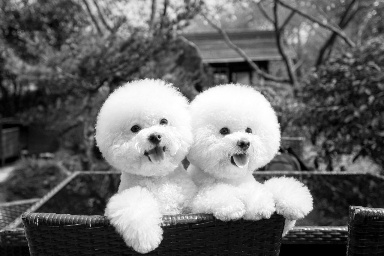
\includegraphics[width=0.5\textwidth]{red_channel.jpg}
  \caption{Red Channel of Image 1}
  \label{fig:example}
\end{figure}

% Refer to the image
The results of the upper operation shown in Figure 1. And analogously, we can show the green and blue channels in Figure 2 and Figure 3.

% Insert an image
\begin{figure}[H]
  \centering
  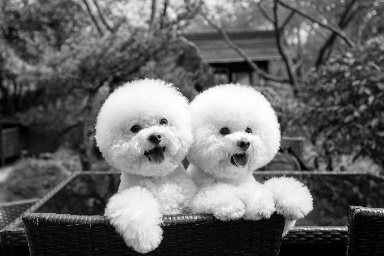
\includegraphics[width=0.5\textwidth]{green_channel.jpg}
  \caption{Green Channel of Image 1}
  \label{fig:example}
\end{figure}

% Insert an image
\begin{figure}[H]
  \centering
  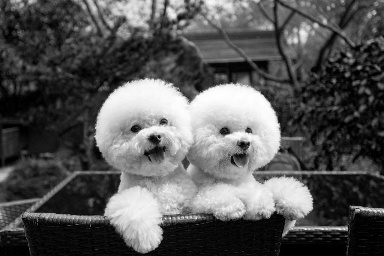
\includegraphics[width=0.5\textwidth]{blue_channel.jpg}
  \caption{Blue Channel of Image 1}
  \label{fig:example}
\end{figure}

\subsubsection{}
\quad According to section 1.2.c in the code file, we can compute and display a histogram for each of the grayscale images.
\begin{python}
  # (c) Compute and display histograms
  def display_histogram(image1, title, color):
  plt.hist(image1.ravel(), 256, [0, 256], color=color, alpha=0.7)
  plt.title(title)

  # Create a figure with three subplots in a single row
  plt.figure(figsize=(12, 4))

  # Display histograms for each channel in a single row with three columns
  plt.subplot(1, 3, 1)
  display_histogram(r, 'Red Channel Histogram', 'red')

  plt.subplot(1, 3, 2)
  display_histogram(g, 'Green Channel Histogram', 'green')

  plt.subplot(1, 3, 3)
  display_histogram(b, 'Blue Channel Histogram', 'blue')

  # Save the combined histogram fugure
  plt.savefig('merged_histogram.png')
  # Show the figure
  plt.show()
\end{python}

\begin{figure}[H]
  \centering
  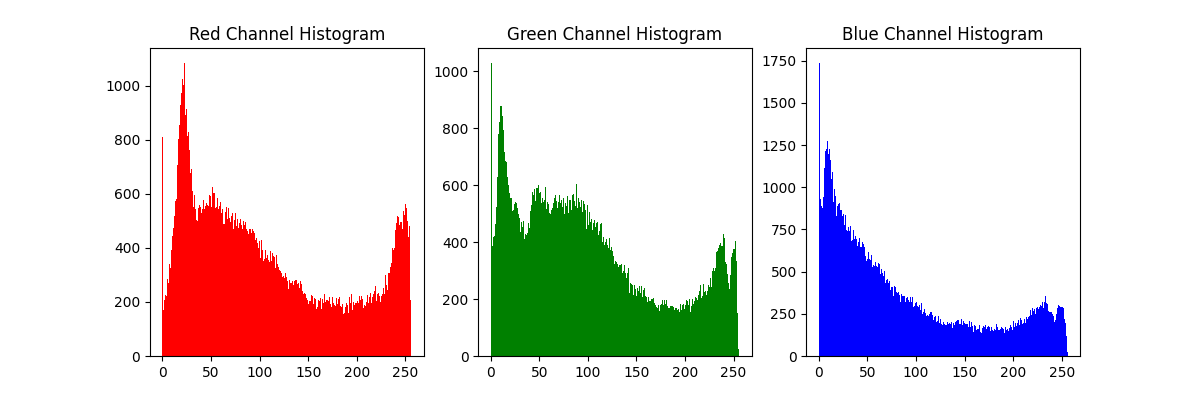
\includegraphics[width=1.0\textwidth]{merged_histogram.png}
  \caption{Histogram of Image 1}
  \label{fig:example}
\end{figure}

\subsubsection{}
\quad As it shows in Figure 4, according to section 1.2.d in the code file, we can generate equalized histogram.
\begin{python}
  # (d) Histogram equalization
  def histogram_equalization(image1):
  # Compute the histogram of the input image with 256 bins in the range [0, 256]
  hist, bins = np.histogram(image1.ravel(), 256, [0, 256])
  # Calculate the cumulative distribution function (CDF) from the histogram
  cdf = hist.cumsum()
  # Normalize the CDF
  cdf_normalized = cdf * hist.max() / cdf.max()
  # Mask the zeros in the CDF to avoid division by zero
  cdf_m = np.ma.masked_equal(cdf, 0)
  # Perform contrast stretching on the masked CDF
  cdf_m = (cdf_m - cdf_m.min()) * 255 / (cdf_m.max() - cdf_m.min())
  # Fill the masked values with zero and convert the result to uint8
  cdf = np.ma.filled(cdf_m, 0).astype('uint8')
  # Use the CDF to create a new equalized image
  img_new = cdf[image1]
  return img_new
\end{python}
\quad We can apply the written function to the image and display the results as Figure 5.
\begin{python}
  # (d) Apply the function and display the histogram equalized image
  b_eq = histogram_equalization(b)
  g_eq = histogram_equalization(g)
  r_eq = histogram_equalization(r)

  # Create a figure with three subplots in a single row
  plt.figure(figsize=(12, 4))

  # Display equalized histograms for each channel in a single row with three columns
  plt.subplot(1, 3, 1)
  display_histogram(r_eq, 'Equalized Red Channel Histogram', 'red')

  plt.subplot(1, 3, 2)
  display_histogram(g_eq, 'Equalized Green Channel Histogram', 'green')

  plt.subplot(1, 3, 3)
  display_histogram(b_eq, 'Equalized Blue Channel Histogram', 'blue')

  # Show the figure
  plt.savefig('equalized_histogram.png')
  plt.show()
\end{python}

\begin{figure}[H]
  \centering
  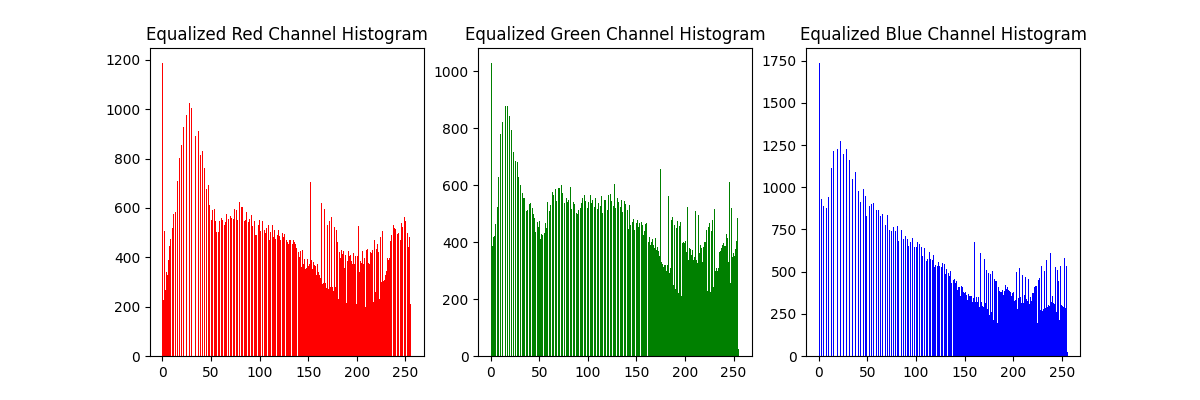
\includegraphics[width=1.0\textwidth]{equalized_histogram.png}
  \caption{Equalized Histogram of Image 1}
  \label{fig:example}
\end{figure}

\section{Task 2: Colour Space Conversion}

\subsection{Question 1}

\subsubsection{}
\quad The HSV values can be computed by the code in section 2.1.a.
\begin{python}
# (a) define my own rgb2hsv function,follow the formula
# The range of pixel intensity can be either 
# [0,255] (if the type of your image is uint8 or integer), 
# or [0,1] (if the type of your image is float)
def cvRGB2HSV(src_r, src_g, src_b):
    r = src_r / 255.0
    g = src_g / 255.0
    b = src_b / 255.0

    h, s, v = 0.0, 0.0, 0.0  # h:0-360.0, s:0.0-1.0, v:0.0-1.0

    color_max = max(r, g, b)
    color_min = min(r, g, b)

    v = color_max

    if color_max == 0.0:
        s = 0
        h = 0
    elif color_max - color_min == 0.0:
        s = 0
        h = 0
    else:
        s = (color_max - color_min) / color_max

        if color_max == r:
            h = 60 * ((g - b) / (color_max - color_min)) + 0
        elif color_max == g:
            h = 60 * ((b - r) / (color_max - color_min)) + 120
        else:
            h = 60 * ((r - g) / (color_max - color_min)) + 240

    if h < 0:
        h += 360.0

    dst_h = int(h / 2)   # dst_h : 0-180
    dst_s = int(s * 255)  # dst_s : 0-255
    dst_v = int(v * 255)  # dst_v : 0-255

    return dst_h, dst_s, dst_v
\end{python}
\subsubsection{}
\quad Read in Figure 2(a) and convert it with my own written function (as it shows in Figure 6), and then display the H, S, and V
channels as follows in Figure 7.
\begin{python}
# Read Figure 2(a)
image_path = "Figure2-a.png"  # Replace with the actual path
image2 = cv2.imread(image_path)

# Extract individual color channels
b, g, r = cv2.split(image2)

# Convert RGB to HSV using custom function
h, s, v = np.vectorize(cvRGB2HSV)(r, g, b)

# Merge h, s, v channels
hsv_result = cv2.merge([h, s, v])
plt.imshow(hsv_result)
plt.imshow(hsv_result)
\end{python}

\begin{figure}[H]
  \centering
  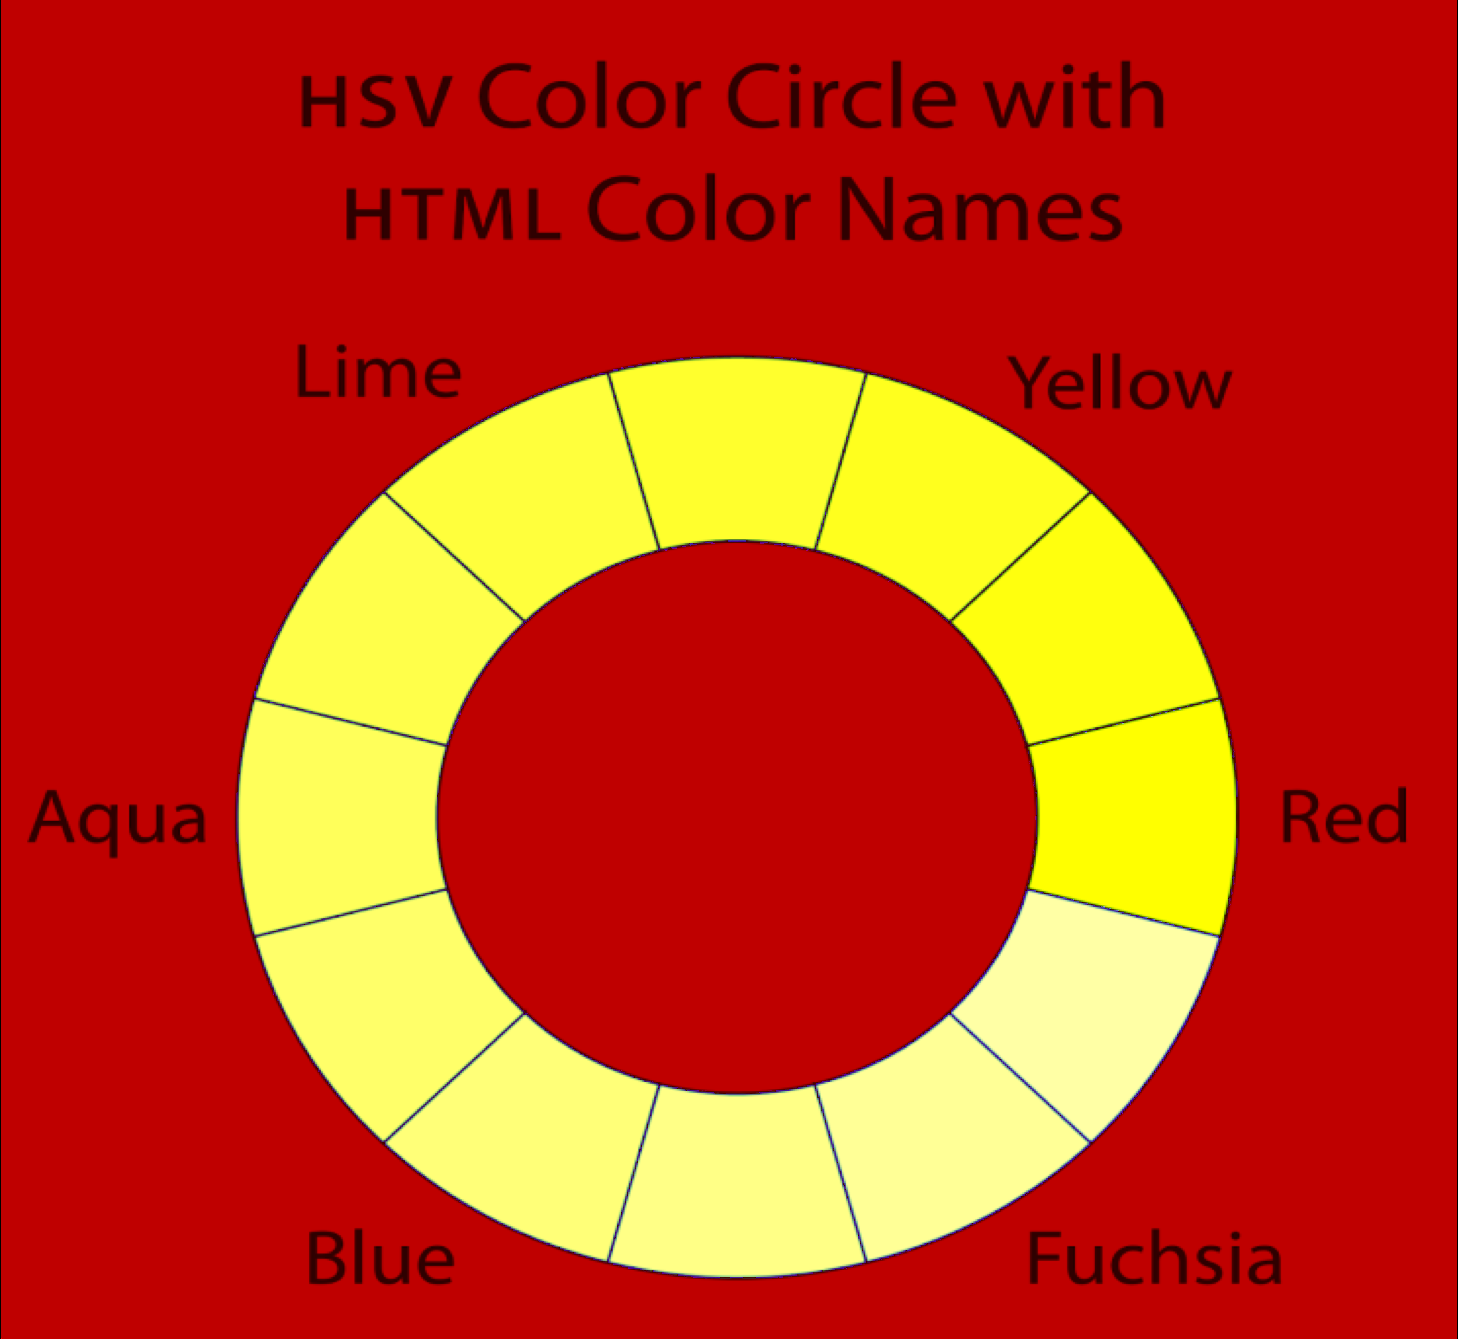
\includegraphics[width=0.5\textwidth]{hsv_result.png}
  \caption{HSV Image of Figure 2(a)}
  \label{fig:example}
\end{figure}

\begin{python}
# Display H, S, V channels
plt.figure(figsize=(12, 4))

plt.subplot(1, 3, 1)
plt.imshow(h, cmap='hsv')
plt.title('Hue (H)')
plt.axis('off')

plt.subplot(1, 3, 2)
plt.imshow(s, cmap='hsv')
plt.title('Saturation (S)')
plt.axis('off')

plt.subplot(1, 3, 3)
plt.imshow(v, cmap='hsv')
plt.title('Value (V)')
plt.axis('off')

plt.savefig('hsv_channels.png')
plt.show()
\end{python}

\begin{figure}[H]
  \centering
  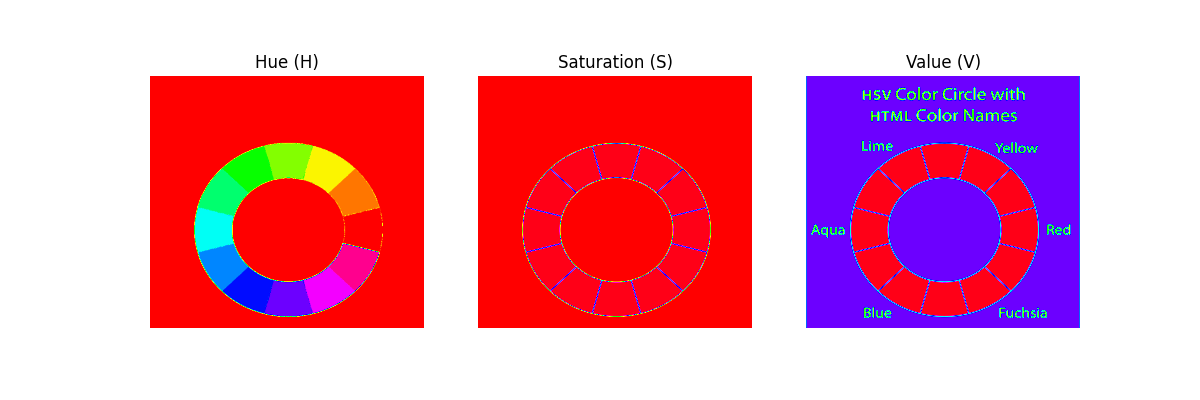
\includegraphics[width=1.0\textwidth]{hsv_channels.png}
  \caption{H, S, V Channels of Figure 2(a)}
  \label{fig:example}
\end{figure}

\subsection{Question 2}

\subsubsection{}
The Hue value is \dots
\subsubsection{}
\quad To solve the given question, we have to at first figure out the edges of each part of the image. The code in section 2.2.a can be used to achieve this. As it is showed in Figure 8, we can get the edges of the image.
\begin{python}
# Load the image
image = Image.open("Figure2-b.png")

# Convert the image to a NumPy array
image_array = np.array(image)

# Find edges using the Sobel operator
# Continuing reduce the high threshold value until all edges visible
import cv2
edges = cv2.Canny(image_array, 100, 160)

# Display the edges
edges_image = Image.fromarray(edges)
edges_image.show()
edges_image.save('edges.png')
  \end{python}

\begin{figure}[H]
  \centering
  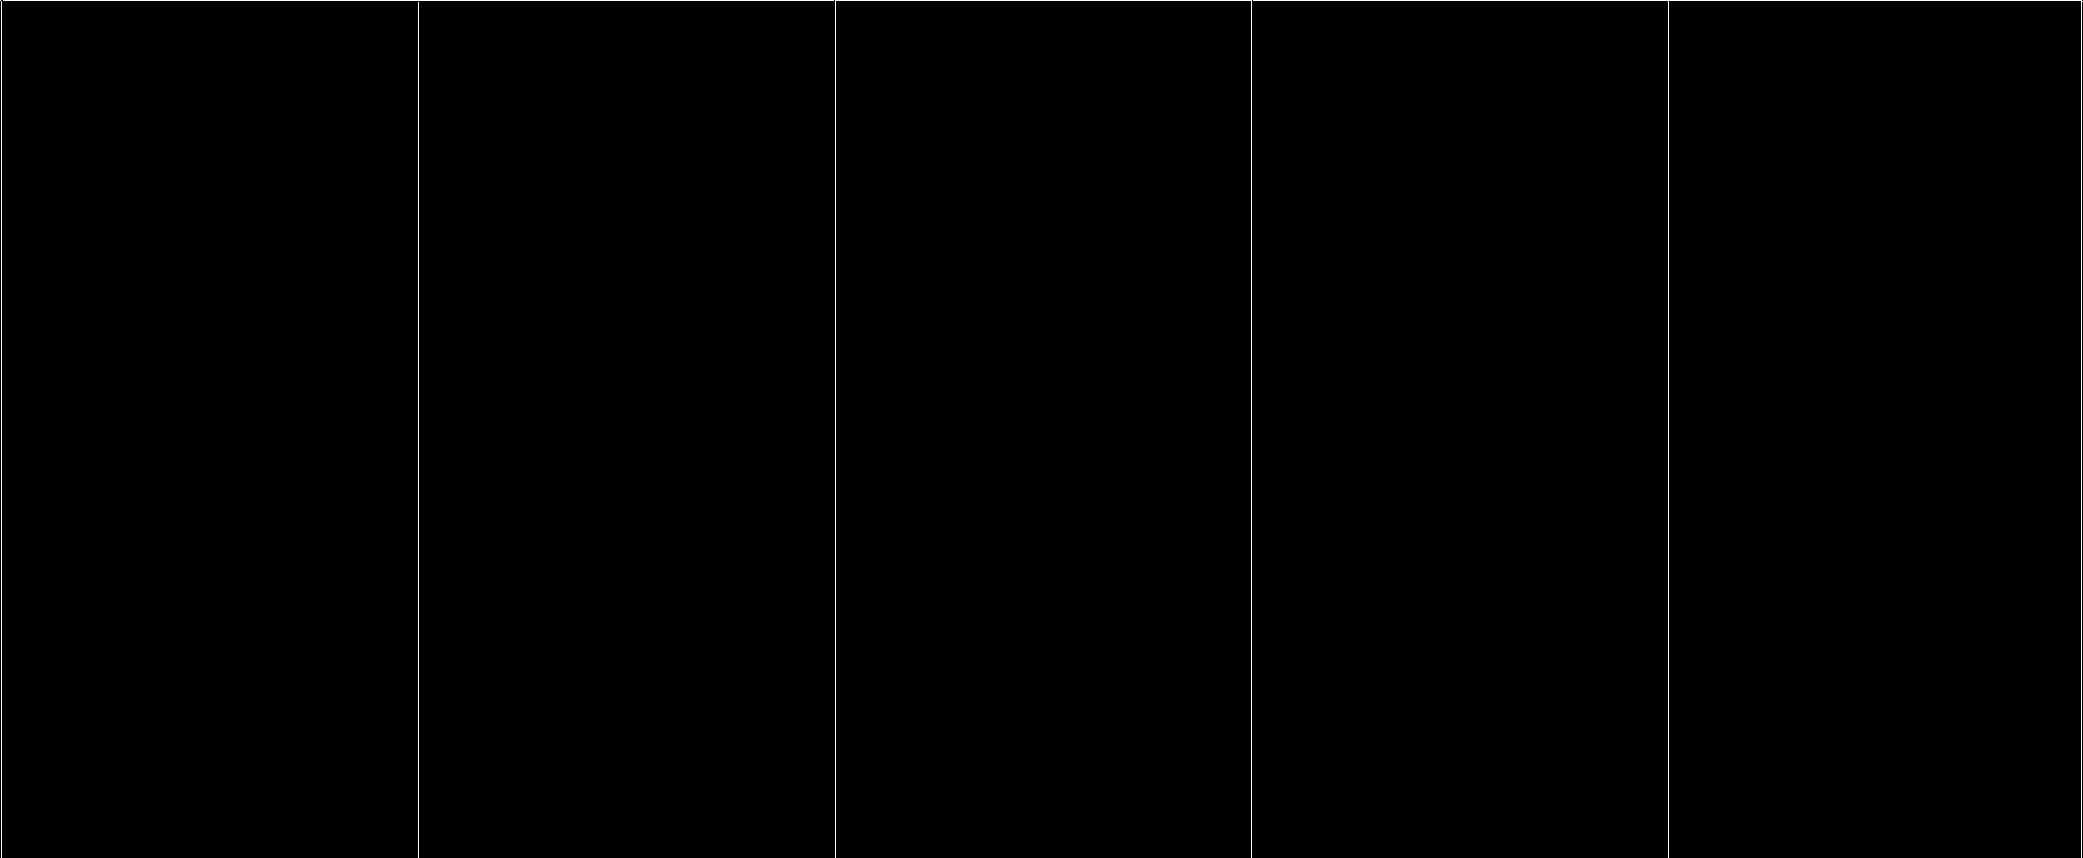
\includegraphics[width=1.0\textwidth]{edges.png}
  \caption{Edges of Figure 2(b)}
  \label{fig:example}
\end{figure}

\section{Task 3: Image Denoising via a Gaussian Filter}

\subsection{Question 1}

\quad I have found that using Haar feature-based cascade classifiers for object detection (mostly used in human face detection) is an effective approach. This method was proposed by Paul Viola and Michael Jones in their 2001 paper "Rapid Object Detection using a Boosted Cascade of Simple Features." It is a machine learning-based approach where a cascade function is trained from a large number of positive and negative images and then applied to detect objects in other images. I applied this method to cat face detection and found that the built-in function worked well. Check the 3.1 section in the code file for it. The original image is displayed in Figure 9 and the resized one in Figure 10.
\begin{python}
# Load the image
image = cv2.imread('image4.jpg')

# Convert to grayscale
gray = cv2.cvtColor(image, cv2.COLOR_BGR2GRAY)

# Detect the cat's face
face_cascade = cv2.CascadeClassifier(cv2.data.haarcascades + 'haarcascade_frontalcatface_extended.xml')
faces = face_cascade.detectMultiScale(gray, scaleFactor=1.1, minNeighbors=5, minSize=(30, 30))

# Assuming there's only one cat face in the image
if len(faces) > 0:
    # Get the coordinates of the face
    (x, y, w, h) = faces[0]
    
    # Calculate the center and the square size
    center_x = x + w // 2
    center_y = y + h // 2
    square_size = max(w, h)
    
    # Calculate the coordinates of the square region
    left = center_x - square_size // 2
    top = center_y - square_size // 2
    right = left + square_size
    bottom = top + square_size
    
    # Crop the square region and resize it to 512x512
    cropped = gray[top:bottom, left:right]
    resized = cv2.resize(cropped, (512, 512))
    
    # Save the resized grayscale image
    cv2.imwrite('cropped_cat_face.jpg', resized)
    
    # Display the original and cropped images
    cv2.imshow('Original', image)
    cv2.imshow('Cropped Cat Face', resized)
    cv2.waitKey(0)
    cv2.destroyAllWindows()
else:
    print('No cat face detected in the image.')
    \end{python}

    \begin{figure}[H]
      \centering
      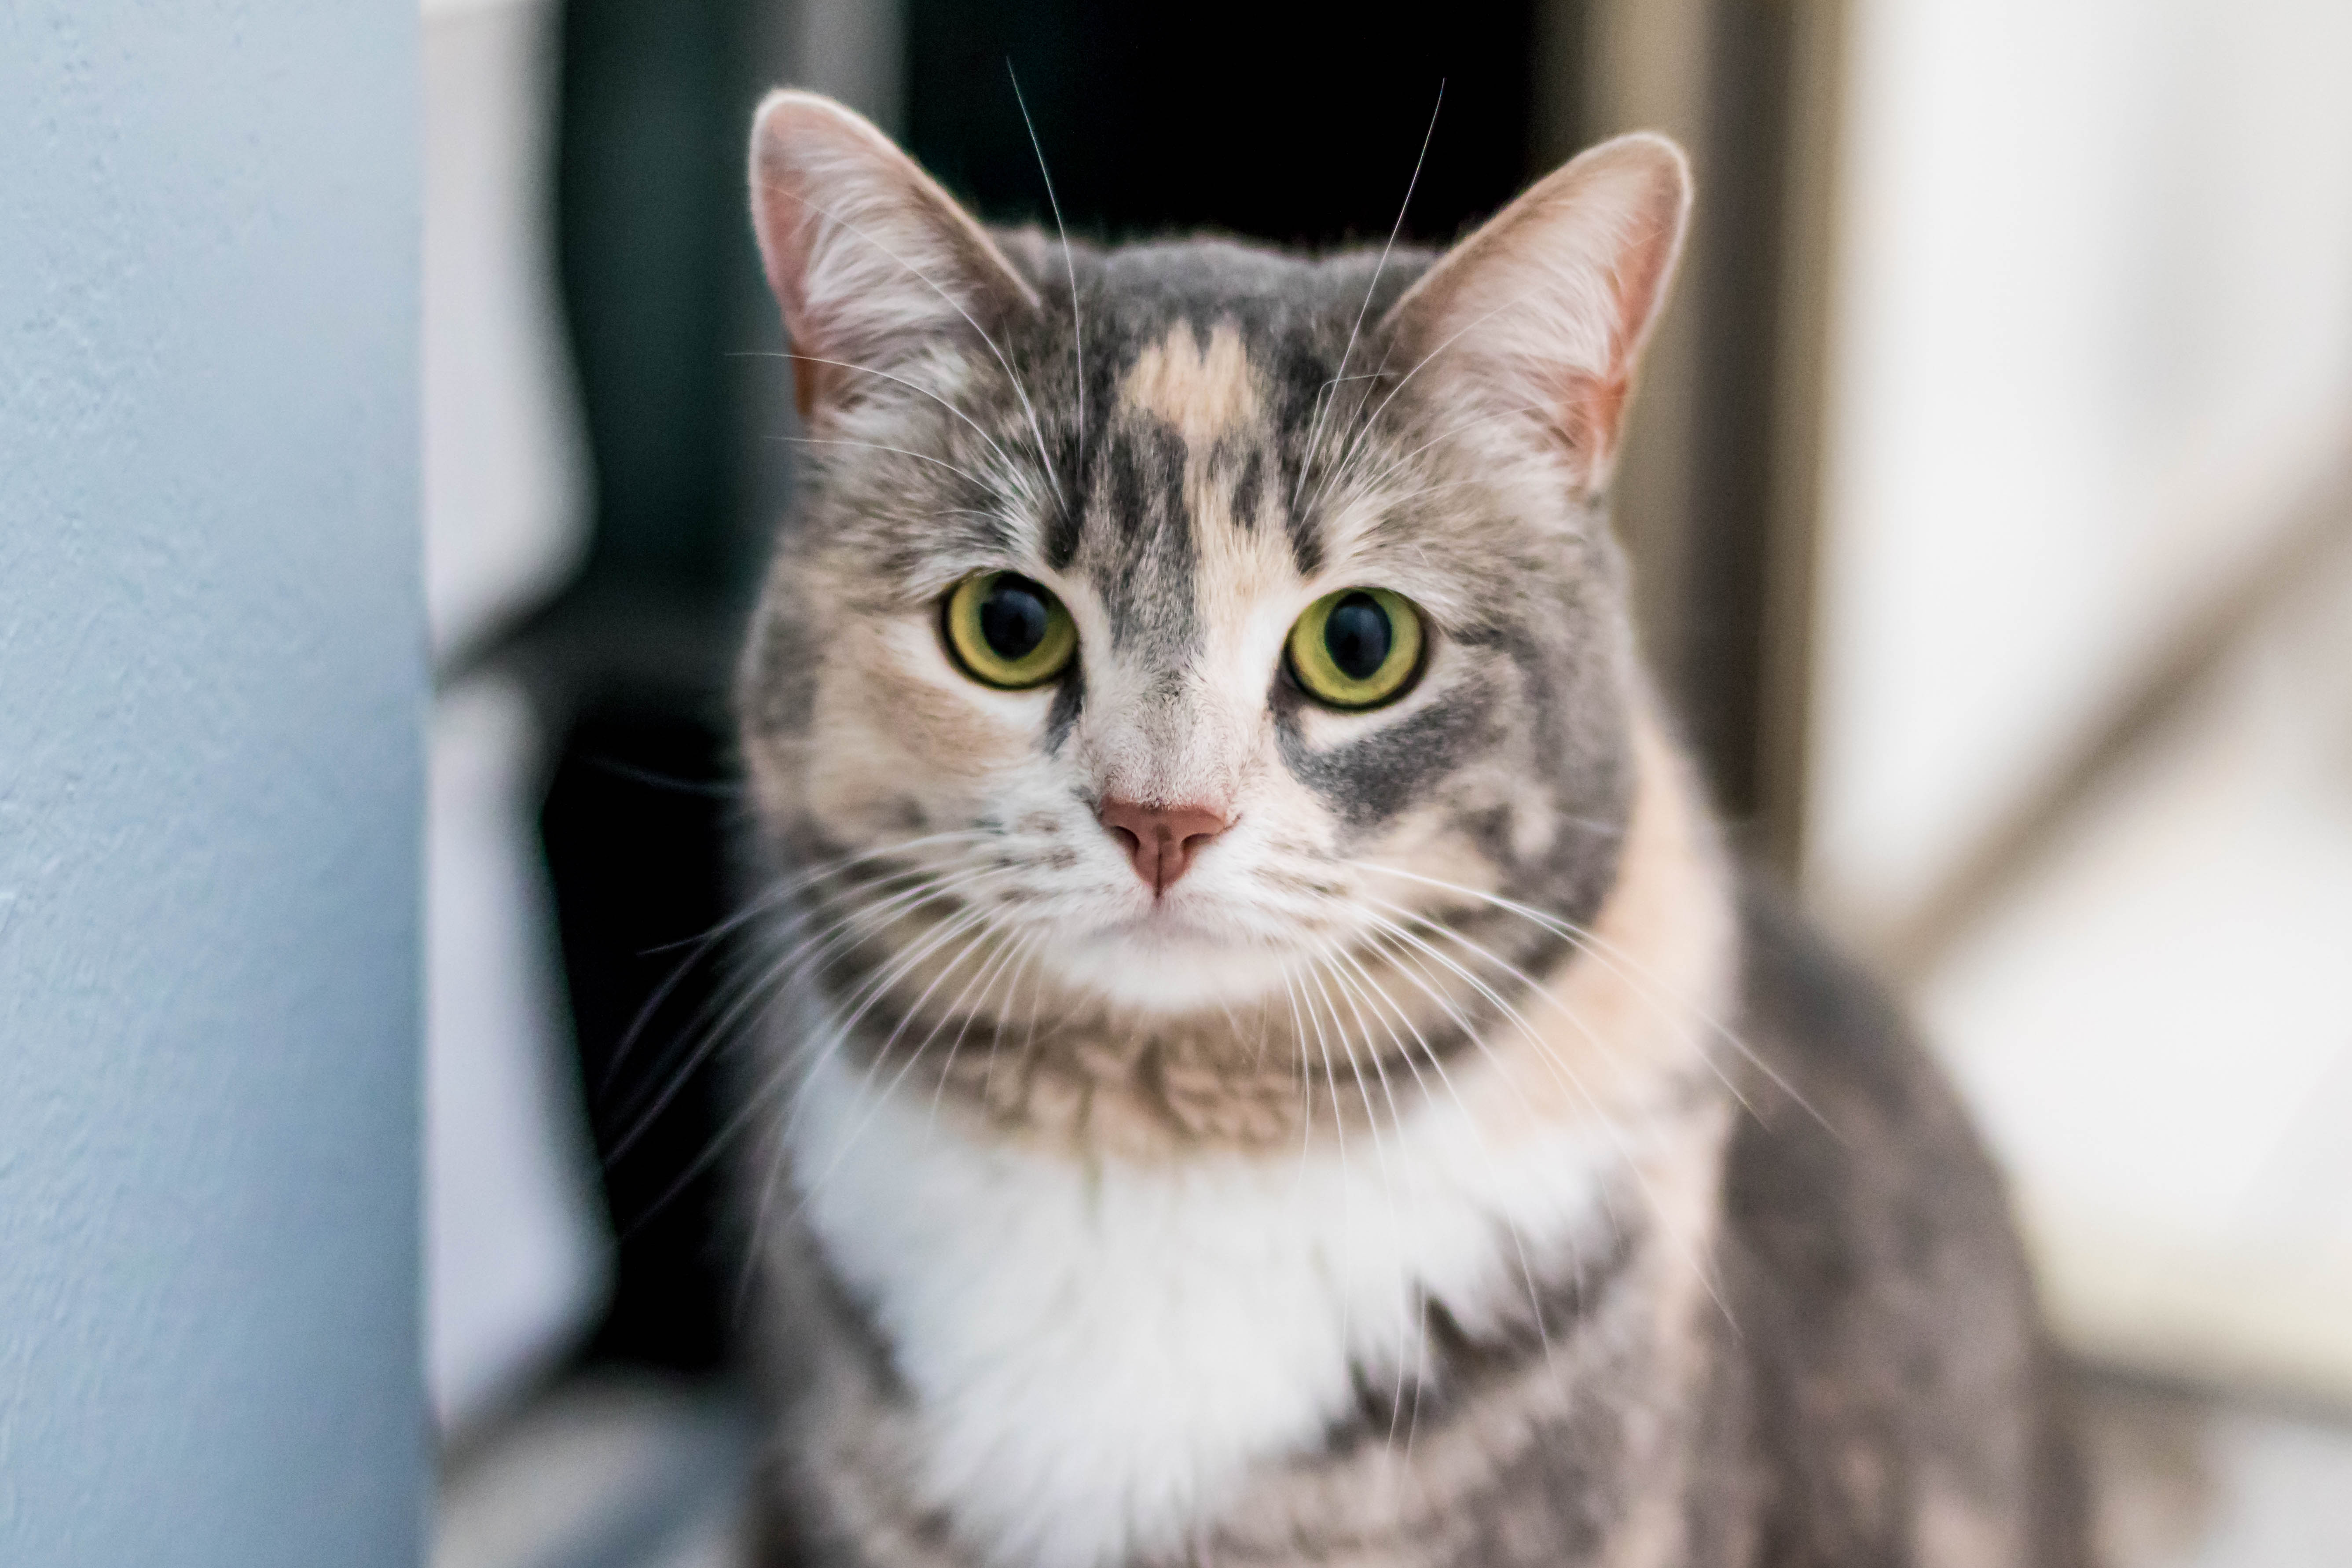
\includegraphics[width=1.0\textwidth]{image4.jpg}
      \caption{Original Image 4}
      \label{fig:example}
    \end{figure}

    \begin{figure}[H]
      \centering
      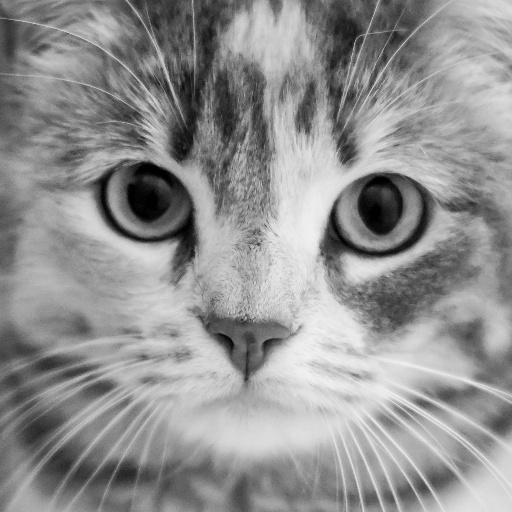
\includegraphics[width=0.5\textwidth]{cropped_cat_face.jpg}
      \caption{Resized Image 4}
      \label{fig:example}
    \end{figure}

\subsection{Question 2}
\quad According the code in section 3.2, we can add Gaussian noise to the resized image and save the noisy image as a new file (Figure 11 as shows). The code is as follows.
\begin{python}
# Add Gaussian noise with zero mean and standard deviation of 15
# * is the syntax for unpacking the (height, width) tuple
# *resized.shape is equivalent to writing height, width 
noise = np.random.randn(*resized.shape) * 15
noisy_image = resized + noise.astype(np.int8)
    
# Clip the intensity values to be within [0, 255]
noisy_image = np.clip(noisy_image, 0, 255).astype(np.uint8)
         
# Save the noisy image
cv2.imwrite('noisy_cat_face.jpg', noisy_image)

\end{python}

\begin{figure}[H]
  \centering
  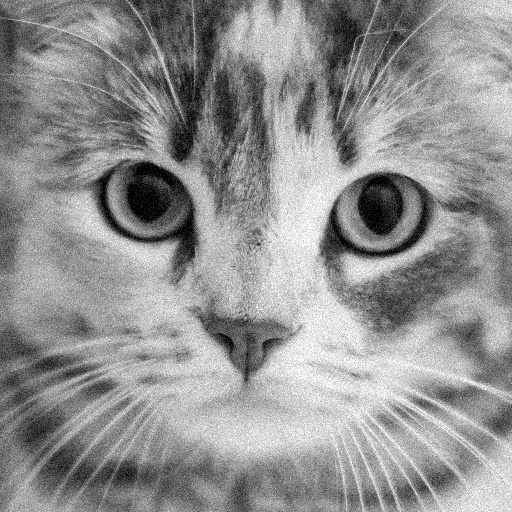
\includegraphics[width=0.5\textwidth]{noisy_cat_face.jpg}
  \caption{Noisy Cat Face}
  \label{fig:example}
\end{figure}

\subsection{Question 3}
\quad By the following code in section 3.3, we can compute and display two intensity histograms as Figure 12.

\begin{python}
  # Compute and display histograms
plt.subplot(121)
plt.hist(resized.ravel(), 256, [0, 256])
plt.title('Original Image Histogram')

plt.subplot(122)
plt.hist(noisy_image.ravel(), 256, [0, 256])
plt.title('Noisy Image Histogram')

plt.savefig('original_and_noisy_histograms.png')
plt.show()
\end{python}

\begin{figure}[H]
  \centering
  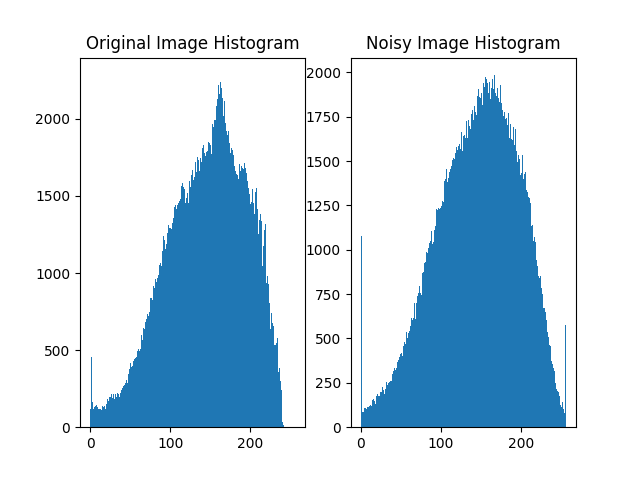
\includegraphics[width=1.0\textwidth]{original_and_noisy_histograms.png}
  \caption{Original and Noisy Image Histograms}
  \label{fig:example}
\end{figure}

\quad As it is shown in Figure 12 (please note that the vertical axis scales are not the same.), the histogram on the left represents the original image before adding noise, while the histogram on the right shows the image after adding noise. Both histograms have a similar unimodal distribution, with a single prominent peak around the grayscale intensity value of approximately 100. However, there are some noticeable differences:\\
- Peak height: The peak in the noisy image histogram is slightly lower than the original one. This suggests that the noise addition has caused some dispersion of the intensity values around the peak.\\
- Spread: The spread of the intensity values in the noisy image histogram is wider than the original one, which indicates noise has introduced a wider range of intensity values, deviating from the concentrated peak in the original image.\\
\\
The overall similarity in the unimodal distribution shape between the two histograms suggests that the added noise did not significantly alter the overall intensity characteristics of the image. However, the differences in peak height, spread indicate that the noise addition has introduced some variations and deviations from the original intensity distribution, as expected when adding random noise to an image.
\subsection{Question 4}
\quad The folowing code in section 3.4 can be used to apply a Gaussian filter to the noisy image and display the filtered image as Figure 13.
\begin{python}
  def my_Gauss_filter(noisy_image, my_7x7_gauss_kernel):
    # Get the size of the kernel
    kernel_size = my_7x7_gauss_kernel.shape[0]
    # Get the border size for symmetric padding
    border_size = kernel_size // 2

    # Pad the noisy image with symmetric padding
    padded_image = cv2.copyMakeBorder(noisy_image, border_size, border_size, border_size, border_size, cv2.BORDER_REFLECT)

    # Initialize the output image
    output_image = np.zeros_like(noisy_image, dtype=np.float32)

    # Apply the 7x7 Gaussian filter
    for i in range(border_size, padded_image.shape[0] - border_size):
        for j in range(border_size, padded_image.shape[1] - border_size):
            patch = padded_image[i - border_size:i + border_size + 1, j - border_size:j + border_size + 1]
            weighted_sum = np.sum(patch * my_7x7_gauss_kernel)
            output_image[i - border_size, j - border_size] = weighted_sum

    # Clip the values to be within [0, 255] range
    output_image = np.clip(output_image, 0, 255).astype(np.uint8)

    return output_image
\end{python}

\subsection{Question 5}
\quad To apply the gaussian filter to the noisy image, we should at first generate kernel and then apply the filter. The code in section 3.5 can be used to achieve this. Noisy image and filtered image is shown in Figure 13.
\begin{python}
# Size of the kernel
kernel_size = 3
# Standard deviation of the Gaussian distribution
std_dev = 0.8

# Generate a 1D Gaussian kernel
my_7_gaussian_kernel = cv2.getGaussianKernel(kernel_size,std_dev)
print(my_7_gaussian_kernel)

# Convert the 1D kernel to a 2D kernel
my_7x7_gauss_kernel = np.outer(my_7_gaussian_kernel, my_7_gaussian_kernel )
print(my_7x7_gauss_kernel)
# Normalize the kernel to make sure the sum of elements is 1
# Seems that this step is not necessary specifically because I have already use the cv2.getGaussianKernel and the originial kernel is already normalized. However, the result does not change if I normalize it again.
my_7x7_gauss_kernel /= my_7x7_gauss_kernel.sum()
----------------------------------------------------------------
# Apply your Gaussian filter
filtered_image = my_Gauss_filter(noisy_image, my_7x7_gauss_kernel)

# Save the filtered image
cv2.imwrite('filtered_cat_face.jpg', filtered_image)

# Display the results
plt.figure(figsize=(10, 5))
plt.subplot(1, 2, 1)
plt.imshow(noisy_image, cmap='gray')
plt.title('Noisy Image')
plt.axis('off')

plt.subplot(1, 2, 2)
plt.imshow(filtered_image, cmap='gray')
plt.title('Filtered Image')
plt.axis('off')

plt.show()
\end{python}

\begin{figure}[H]
  \centering
  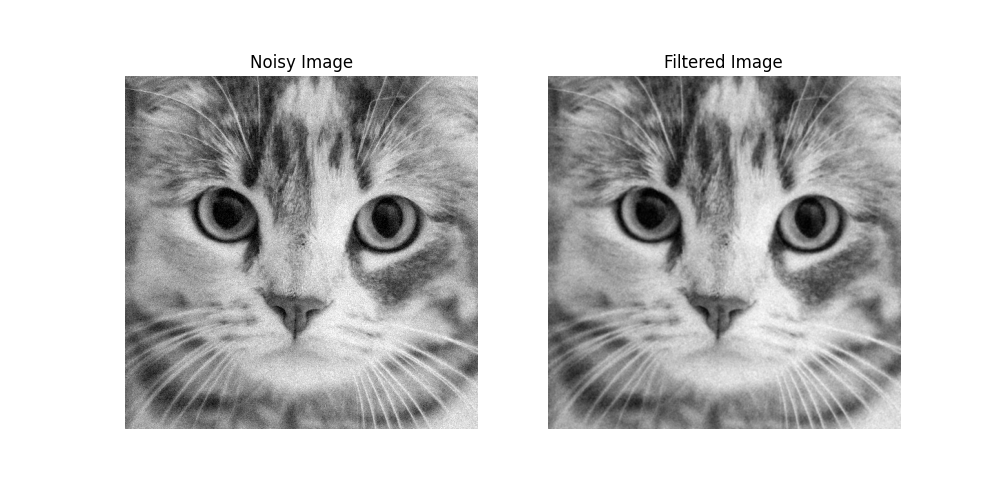
\includegraphics[width=1.0\textwidth]{noisy_and_filtered_cat_face.png}
  \caption{Filtered Cat Face}
  \label{fig:example}
\end{figure}

\quad As it is shown in Figure 13, can visually observe that the filtered image appears smoother and has reduced noise levels. The details and features of the cat's face are preserved, but the graininess and pixel-level distortions have been effectively smoothed out by the Gaussian filter. The filtered image has a more uniform and consistent appearance, with less visible noise artifacts compared to the noisy image. This demonstrates the effectiveness of the Gaussian filter in reducing noise and improving the overall visual quality of the image.
\subsection{Question 6}
\quad As it said in the question, one of the key parameters to choose for the task of image filtering is the standard deviation. We are now going to investigate the effect of the standard deviation on the filtering process by comparing the differences images generated by different standard deviation according to the code in section 3.6.

\begin{python}

# Define the size of the Gaussian kernel
kernel_size = 7

# Generate a range of standard deviations to test
std_devs = [1.0, 10.0, 100.0]

# Display the images in a 4x2 grid
plt.figure(figsize=(12, 16))

# Display the original image in the first column
plt.subplot(4, 2, 1)
plt.imshow(noisy_image, cmap='gray')
plt.title('Original Image')
plt.axis('off')

plt.subplot(4, 2, 8)
plt.imshow(noisy_image, cmap='gray')
plt.title('Original Image')
plt.axis('off')

# Iterate through different standard deviations
for i, std_dev in enumerate(std_devs):
    # Generate a 1D Gaussian kernel
    gaussian_kernel_1d = gaussian(kernel_size, std=std_dev)

    # Convert the 1D kernel to a 2D kernel
    gaussian_kernel_2d = np.outer(gaussian_kernel_1d, gaussian_kernel_1d)

    # Normalize the kernel
    gaussian_kernel_2d /= gaussian_kernel_2d.sum()

    # Apply your Gaussian filter
    filtered_image = my_Gauss_filter(noisy_image, gaussian_kernel_2d)

    # Display the original image in the second column
    plt.subplot(4, 2, i * 2 + 2)
    plt.imshow(noisy_image, cmap='gray')
    plt.title('Original Image')
    plt.axis('off')

    # Display the filtered image in the second column
    plt.subplot(4, 2, i * 2 + 3)
    plt.imshow(filtered_image, cmap='gray')
    plt.title(f'Std Dev = {std_dev}')
    plt.axis('off')

plt.savefig('gaussian_filter_comparison.png')
plt.show()

\end{python}

\begin{figure}
  \centering
  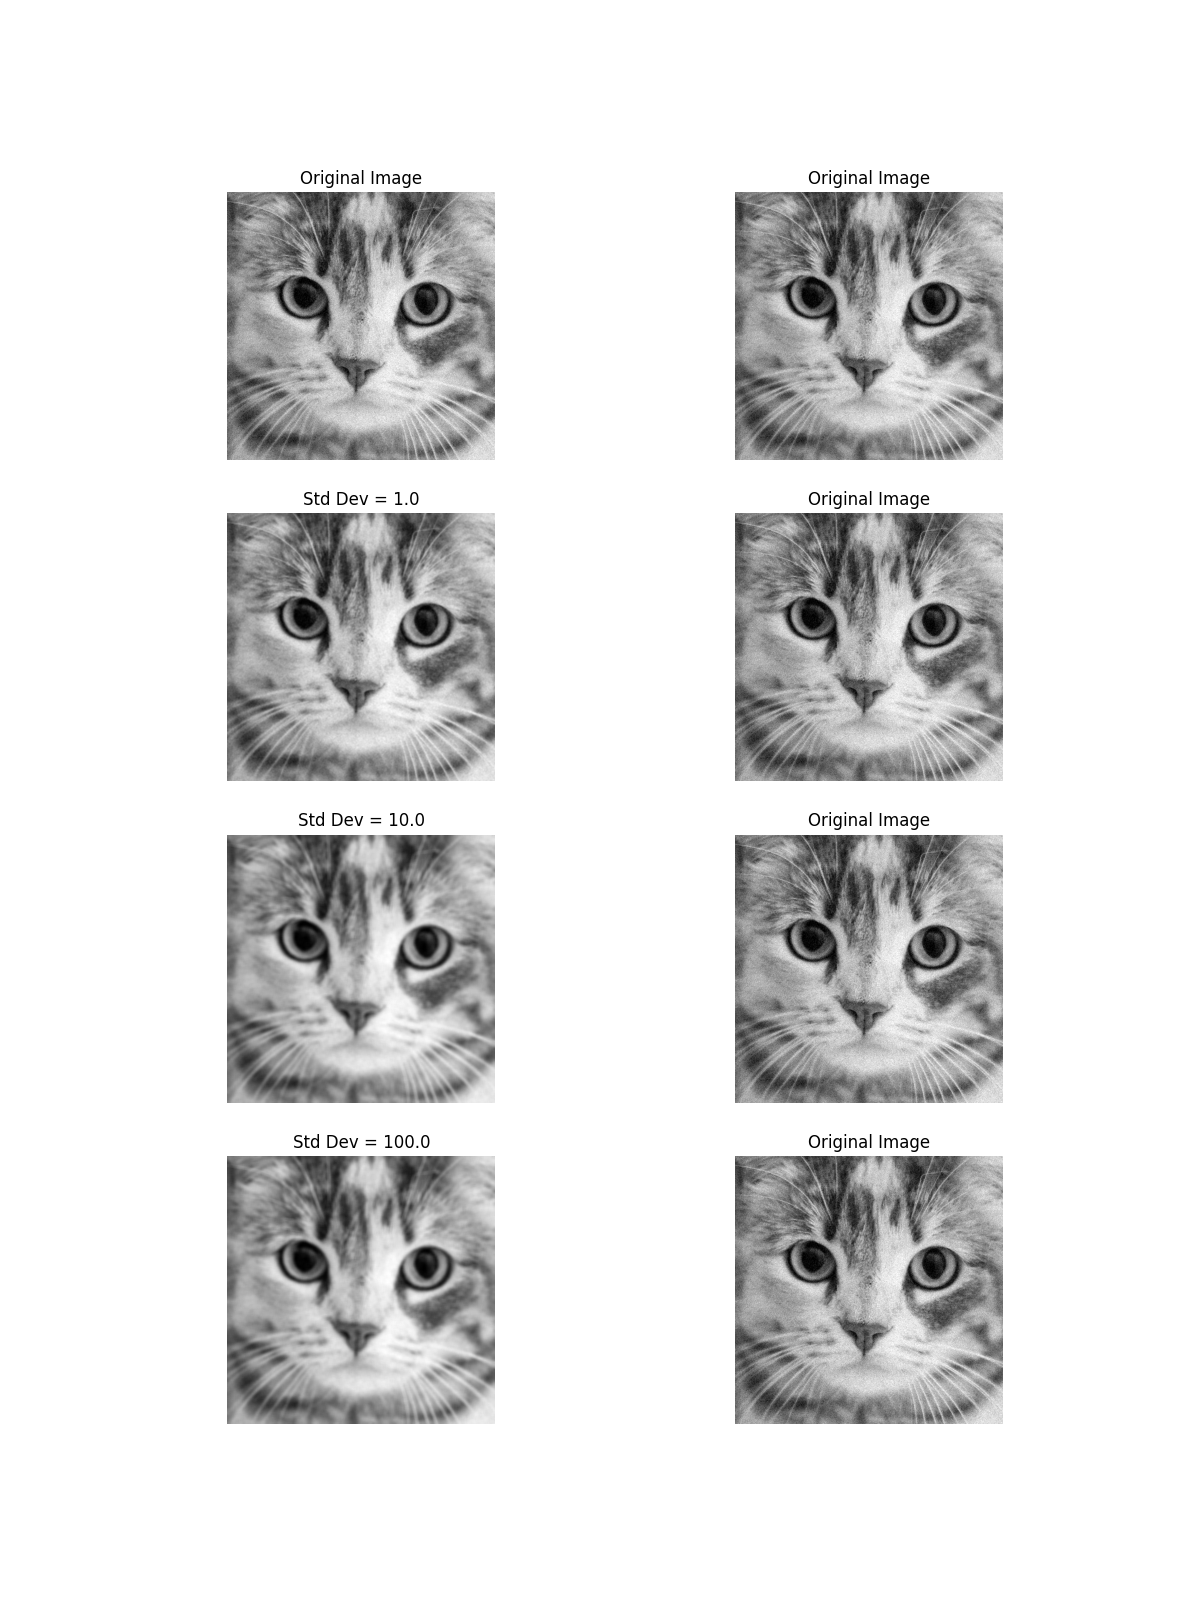
\includegraphics[width=1.0\textwidth]{gaussian_filter_comparison.png}
  \caption{Gaussian Filter Comparison}
  \label{fig:example}
\end{figure}

As it is shown in Figure 14, we can observe the following effects of different standard deviations on the filtering process:\\
The standard deviation parameter controls the degree of smoothing or blurring applied by the Gaussian filter. As the standard deviation value increases, the Gaussian filter applies stronger smoothing, effectively removing more noise but also progressively losing finer details and textures in the process. The choice of the optimal standard deviation depends on the specific application and the desired balance between noise reduction and detail preservation. \\
- Low standard deviation (e.g., 1.0): The filtered image appears to be relatively smooth, with a noticeable reduction in noise levels. However, the details and features of the cat's face are preserved, and the overall appearance of the image is visually similar to the original noisy image.\\
- Moderate standard deviation (e.g., 10.0): The filtered image appears to be smoother and has a more uniform appearance compared to the original noisy image. The noise levels are further reduced, and the overall visual quality of the image is improved.\\
- High standard deviation (e.g., 100.0): The filtered image appears to be excessively smooth, with a significant loss of details and features in the cat's face. The noise levels are effectively reduced, but the image appears to be overly blurred and lacks the sharpness and clarity present in the original noisy image.\\
\subsection{Question 7}
\quad Following the code in section 3.7, we are able to compare the differences between my filter function and the built-in function GaussianBlur() in OpenCV.
\begin{python}
# Define the size of the Gaussian kernel
kernel_size = 7

# Choose a standard deviation for your custom Gaussian filter
std_dev_custom = 2.0

# Generate the 7x7 Gaussian kernel for your custom filter
gaussian_kernel_1d_custom = gaussian(kernel_size, std=std_dev_custom)
gaussian_kernel_2d_custom = np.outer(gaussian_kernel_1d_custom, gaussian_kernel_1d_custom)
gaussian_kernel_2d_custom /= gaussian_kernel_2d_custom.sum()

# Apply your custom Gaussian filter
filtered_image_custom = my_Gauss_filter(noisy_image, gaussian_kernel_2d_custom)

# Apply the built-in Gaussian filter (cv2.GaussianBlur)
filtered_image_opencv = cv2.GaussianBlur(noisy_image, (kernel_size, kernel_size), std_dev_custom)

# Display the results side by side
plt.figure(figsize=(12, 6))

plt.subplot(1, 3, 1)
plt.imshow(noisy_image, cmap='gray')
plt.title('Original Image')
plt.axis('off')

plt.subplot(1, 3, 2)
plt.imshow(filtered_image_custom, cmap='gray')
plt.title('Custom Gaussian Filter')
plt.axis('off')

plt.subplot(1, 3, 3)
plt.imshow(filtered_image_opencv, cmap='gray')
plt.title('cv2.GaussianBlur')
plt.axis('off')

plt.savefig('custom_vs_opencv_gaussian_filter.png')
plt.show()

plt.figure(figsize=(12, 4))

# Compare the two filtered images
difference_image = np.abs(filtered_image_custom - filtered_image_opencv)
threshold = 10  # Adjust the threshold as needed

# Set pixels to white where the difference is below the threshold
difference_image[difference_image < threshold] = 255
plt.subplot(1, 2, 1)
plt.imshow(difference_image, cmap='gray')
plt.title('Difference')
plt.axis('off')

plt.subplot(1, 2, 2)
plt.plot(filtered_image_custom[256, :], label='Custom Filter')
plt.plot(filtered_image_opencv[256, :], label='cv2.GaussianBlur')
plt.title('Pixel Values along Row 256')
plt.legend()

plt.savefig('custom_vs_opencv_gaussian_filter_comparison.png')
plt.show()

\end{python}

\begin{figure}
  \centering
  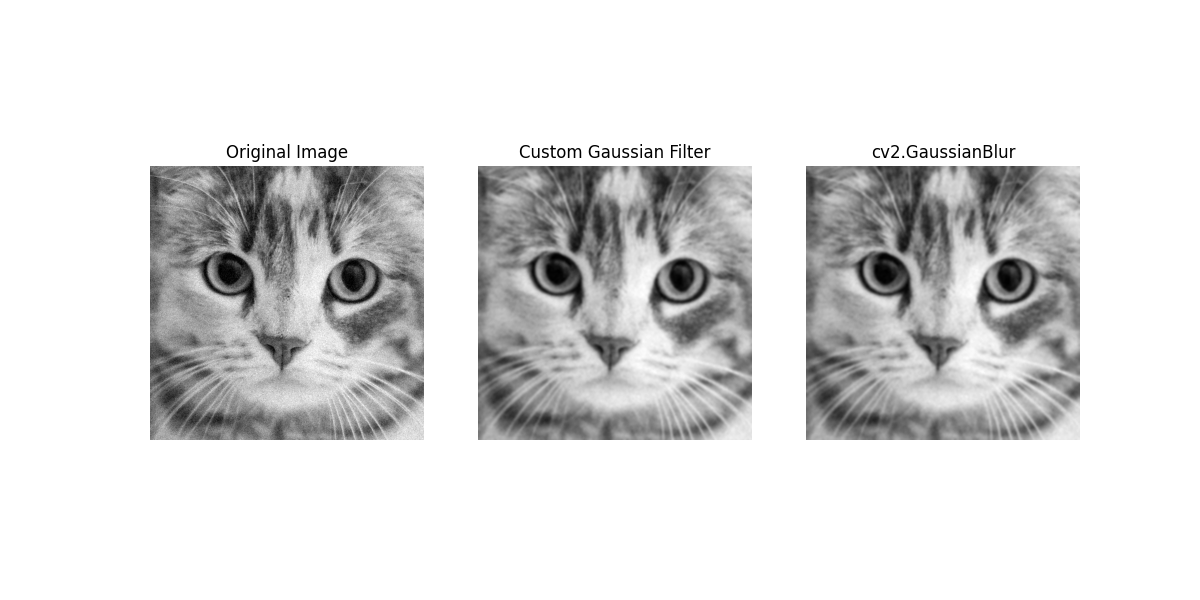
\includegraphics[width=1.0\textwidth]{custom_vs_opencv_gaussian_filter.png}
  \caption{Custom vs. OpenCV Gaussian Filter}
  \label{fig:example}
\end{figure}

\begin{figure}
  \centering
  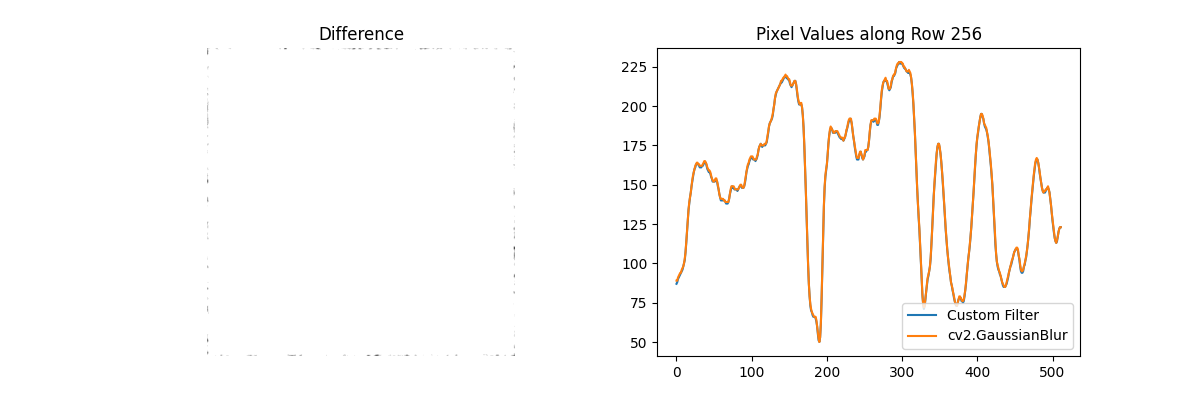
\includegraphics[width=1.0\textwidth]{custom_vs_opencv_gaussian_filter_comparison.png}
  \caption{Custom vs. OpenCV Gaussian Filter Comparison}
  \label{fig:example}
\end{figure}

Figure 15 shows the original image of a cat's face, along with the results of applying two different Gaussian filtering techniques: a custom Gaussian filter and the built-in cv2.GaussianBlur function from OpenCV.\\

Figure 16 provides a visual comparison between the custom Gaussian filter and the OpenCV cv2.GaussianBlur function. The left subplot shows the difference between the two filtered images. The majority of the image appears white, indicating that the difference between the two filtered images is very small.\\

The right subplot plots the pixel values along row 256 of the two filtered images. The two lines (orange and blue) are nearly identical, further confirming that the custom Gaussian filter implementation produces results very similar to the built-in OpenCV function.\\

Based on the provided code and the visual comparisons, it is evident that the custom Gaussian filter implementation yields results that are almost identical to the cv2.GaussianBlur function from OpenCV. The minor differences that may exist can be attributed to rounding errors or slight variations in the implementation details.\\

\section{Task 4: Sobel Edge Filter}
\subsection{Question 1}
\quad We can create my own sobel filter and apply it to the images according to the code in section 4.1. The results are shown in Figure 17 and Figure 18.
\begin{python}
def sobel(img):
    h,w=img.shape
    new_img=np.zeros([h,w])
    x_img=np.zeros(img.shape)
    y_img=np.zeros(img.shape)
    # Sobel filter kernels
    sobel_x=np.array([[-1,0,1],[-2,0,2],[-1,0,1]])
    sobel_y=np.array([[-1,-2,-1],[0,0,0],[1,2,1]])
    # Loop through the image pixels, excluding the image edges
    for i in range(h-2):# should it start on 1 to avoid the edge? If so, all the other loops should minus 1 as well
        for j in range(w-2):
             # Apply the Sobel filters to compute gradient in x and y directions
            x_img[i+1,j+1]=abs(np.sum(img[i:i+3,j:j+3]*sobel_x))
            y_img[i+1,j+1]=abs(np.sum(img[i:i+3,j:j+3]*sobel_y))
            new_img[i+1,j+1]=np.sqrt(np.square(x_img[i+1,j+1])+np.square(y_img[i+1,j+1]))

    return np.uint8(new_img)

----------------------------------------------------------------

# Apply custom Sobel filter to the images
image2 = cv2.imread('image2.jpg', cv2.IMREAD_GRAYSCALE)
result_image2_custom_sobel = sobel(image2)

# Apply built-in Sobel filter to the images
result_image2_opencv_sobel_x = cv2.Sobel(image2, cv2.CV_64F, 1, 0, ksize=3)
result_image2_opencv_sobel_y = cv2.Sobel(image2, cv2.CV_64F, 0, 1, ksize=3)
result_image2_opencv_sobel = np.sqrt(result_image2_opencv_sobel_x**2 + result_image2_opencv_sobel_y**2)

# Visualize the results2
plt.figure(figsize=(12, 8))

plt.subplot(1, 3, 1)
plt.imshow(image2, cmap='gray')
plt.title('Original Image 2')
plt.axis('off')

plt.subplot(1, 3, 2)
plt.imshow(result_image2_custom_sobel, cmap='gray')
plt.title('Custom Sobel')
plt.axis('off')

plt.subplot(1, 3, 3)
plt.imshow(result_image2_opencv_sobel, cmap='gray')
plt.title('OpenCV Sobel')
plt.axis('off')

plt.savefig('sobel_filter_comparison_image2.png')
plt.show() 
----------------------------------------------------------------

# Analogically, we can apply the sobel filter to the image4
image4 = cv2.imread('image4.jpg', cv2.IMREAD_GRAYSCALE)

result_image4_custom_sobel = sobel(image4)

result_image4_opencv_sobel_x = cv2.Sobel(image4, cv2.CV_64F, 1, 0, ksize=3)
result_image4_opencv_sobel_y = cv2.Sobel(image4, cv2.CV_64F, 0, 1, ksize=3)
result_image4_opencv_sobel = np.sqrt(result_image4_opencv_sobel_x**2 + result_image4_opencv_sobel_y**2)

plt.subplot(1, 3, 1)
plt.imshow(image4, cmap='gray')
plt.title('Image 4')
plt.axis('off')

plt.subplot(1, 3, 2)
plt.imshow(result_image4_custom_sobel, cmap='gray')
plt.title('Custom Sobel')
plt.axis('off')

plt.subplot(1, 3, 3)
plt.imshow(result_image4_opencv_sobel, cmap='gray')
plt.title('OpenCV Sobel')
plt.axis('off')

plt.savefig('sobel_filter_comparison_image4.png')
plt.show()
  \end{python}

  \begin{figure}
    \centering
    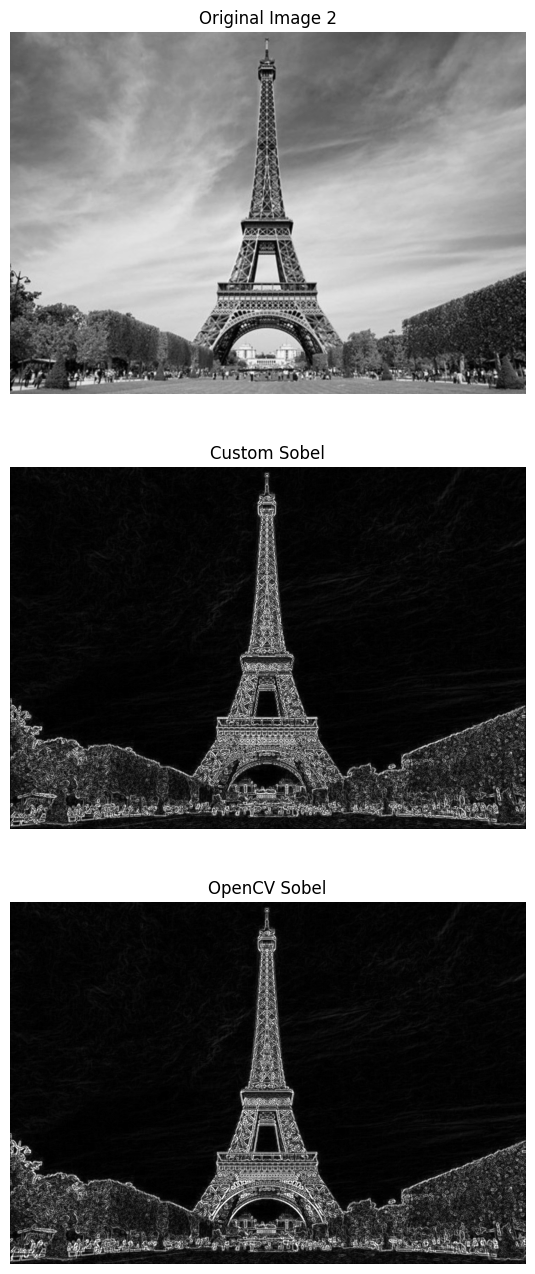
\includegraphics[width=0.5\textwidth]{sobel_filter_comparison_image2.png}
    \caption{Sobel Filter Comparison for Image 2}
    \label{fig:example}
  \end{figure}
  \begin{figure}
    \centering
    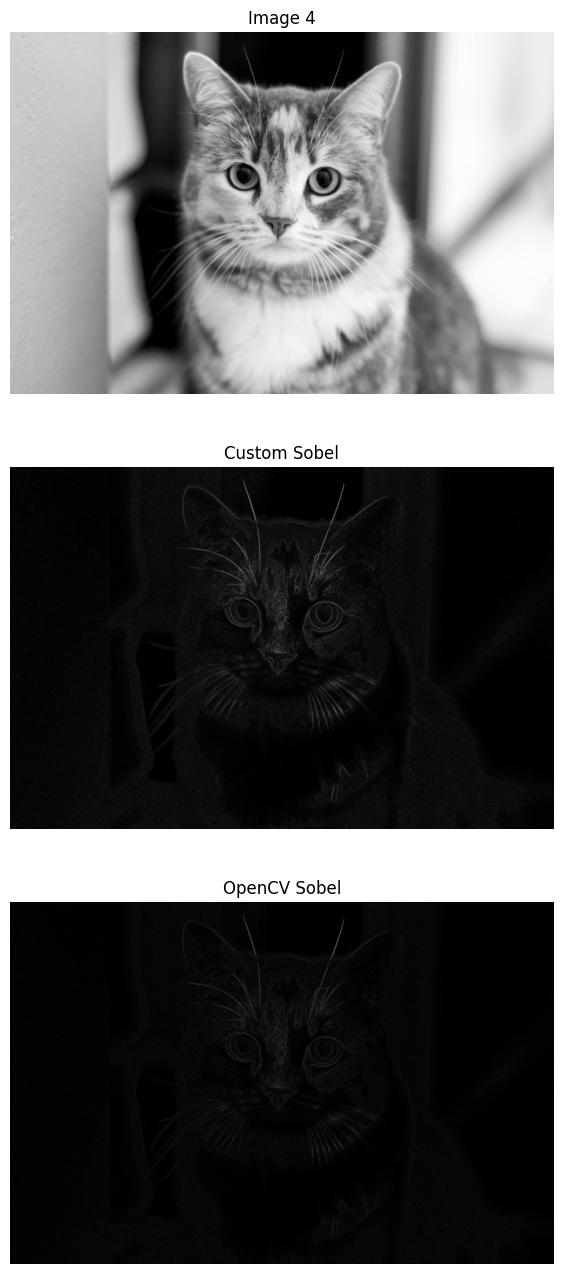
\includegraphics[width=0.5\textwidth]{sobel_filter_comparison_image4.png}
    \caption{Sobel Filter Comparison for Image 4}
    \label{fig:example}
  \end{figure}

  
\subsubsection{}
  As it is shown in Figure 17 and Figure 18, the custom Sobel filter and the built-in OpenCV Sobel filter produce visually different results for the given images. \\
  \\
  For Image 2 (Eiffel Tower), both the Custom Sobel and OpenCV Sobel results appear to correctly detect and highlight the edges of the Eiffel Tower structure, trees, and other elements in the scene.\\
  For Image 4 (Cat), the Custom Sobel result seems to more accurately capture the edges and details of the cat's face and fur compared to the OpenCV Sobel output, which appears too dark and lacks fine details.\\

\subsubsection{}
\quad Sobel filter is a common algorithm used for edge detection in image processing. It works by convolving the image with a pair of NxN kernels to compute the gradient in the x and y directions. The magnitude of the gradient is then used to identify edge pixels in the image.\\
The Sobel filter achieves edge detection by convolving the input image with two separate kernel filters - one for detecting horizontal edges and another for vertical. These kernels apply weighted sums to calculate an approximation of the gradient in each direction. The final output is the combined magnitude of two gradients, which represents the estimated edge strengths and orientations across the image.\\
By emphasizing areas with hrapid intensity changes, the Sobel filter effectively highlights edge regions while suppressing areas with relatively uniform intensities.
\subsection{Question 2}

\quad There are several reasons why the custom Sobel filter might make some inaccuracies prediction. Some is related to the parameters of the filter, the others are related to the images themselves.\\
- Kernel size: The size of the Sobel kernels can affect the sensitivity to noise and the ability to capture fine details. Smaller kernels may be more sensitive to noise, while larger kernels may miss finer details.\\
- Gradient thresholding: The choice of thresholding values for gradient magnitudes can affect the detection of true edges. Setting thresholds too low may result in false positives, while setting them too high may miss true edges.\\
- Noise: Image noise can introduce spurious gradients, leading to inaccurate edge orientation estimations.\\
- Blurring: If the image is blurred, the edges may appear less sharp, affecting the gradient calculations and resulting in inaccurate orientations.\\
- Local variations: The Sobel filter relies on local pixel neighborhoods, so it may struggle with capturing accurate orientations in regions with high local variations or complex textures.\\
- Image artifacts: Non-ideal image conditions, such as lighting variations, shadows, or reflections, can cause the Sobel filter to detect false edges or miss true edges.\\

\quad Using the following code in section 4.2, we can the histogram of the gradient orientation as Figure 19 and Figure 20.
\begin{python}
# Read the image
image_path = "image2.jpg"  # Replace with the actual path
image = cv2.imread(image_path, cv2.IMREAD_GRAYSCALE)

# Calculate gradient in x and y directions
sobelx = cv2.Sobel(image, cv2.CV_64F, 1, 0, ksize=3)
sobely = cv2.Sobel(image, cv2.CV_64F, 0, 1, ksize=3)

# Calculate gradient magnitude and orientation
magnitude = np.sqrt(sobelx**2 + sobely**2)
orientation = np.degrees(np.arctan2(sobely, sobelx)) # Convert radian to degree

# Plot histogram of the gradient orientation
plt.hist(orientation.ravel(), bins=180, range=(0,180))
plt.title('Histogram of Gradient Orientation')
plt.xlabel('Gradient Orientation (degrees)')
plt.ylabel('Frequency')
plt.grid(True)
plt.show()
\end{python}

\begin{figure}
  \centering
  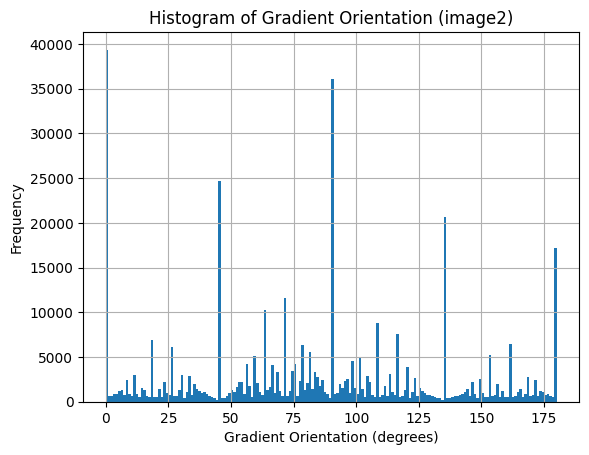
\includegraphics[width=0.5\textwidth]{gradient_orientation_histogram_image2.png}
  \caption{Gradient Orientation Histogram for Image 2}
  \label{fig:example}
\end{figure}

\begin{figure}
  \centering
  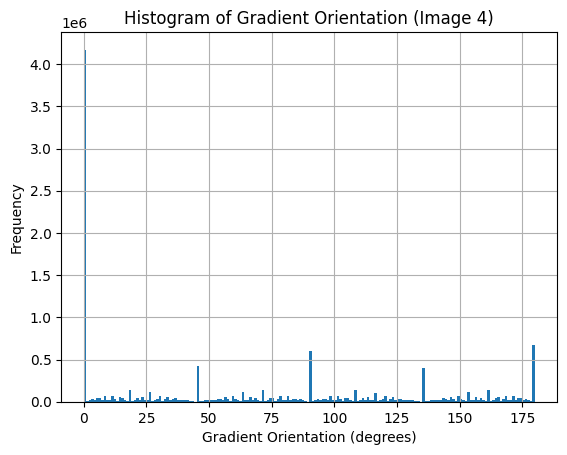
\includegraphics[width=0.5\textwidth]{gradient_orientation_histogram_image4.png}
  \caption{Gradient Orientation Histogram for Image 4}
  \label{fig:example}
\end{figure}

Figure 19 shows the histogram of gradient orientations for image 2, likely calculated using the Sobel filter or a similar edge detection algorithm. The histogram has prominent peaks around 0, 90, and 180 degrees, indicating a significant presence of vertical, horizontal, and diagonal edge orientations in the image. For Image 2, which shows the Eiffel Tower, we would expect to see strong vertical and diagonal edge orientations due to the tower's structure. The histogram in Image 1 aligns well with these expectations, with pronounced peaks around 0 (vertical) and 90 degrees (horizontal/diagonal), indicating that the Sobel filter accurately captured the major edge orientations in this image.\\
\\
\\
Figure 20 show the histogram of gradient orientations for image 4. The prominent peak around 0 degrees corresponds to the darker regions and shadows in the image. The relatively flat distribution across other orientations aligns with the curved and circular shapes of the cat's face. Additionally, the minor peaks in the histogram likely capture straight or diagonal edges from features such as the cat's whiskers and facial markings. The overall distribution in Image 2 provides a reasonable fit for the expected edge orientations in the complex texture and patterns of the cat image.
\section{Task 5: Short Response Questions}

\subsection{Question 1}

\subsubsection{}

\subsubsection{}

\subsection{Question 2}


\subsubsection{}

\subsubsection{}

\subsubsection{}





















% References
\begin{thebibliography}{9}
  \bibitem{example}
  Author,
  \emph{Title}.
  Publisher, Year.
\end{thebibliography}

\end{document}
